\begin{comment}\\
%\newglossaryentry{kiln}
%{
 % name=kiln,
  %description={German: Brennofen (m.);\\Français: fourneau (m.)},
  %plural=kilns
%}

%Make Glossary properly...
%\acrodef{VB}{Visula Basic}
%\makeglossaries
%\newglossaryentry{Availability Zone}
%{
    name=Availability Zone,
    description={Eine Verfügbarkeitszone ist einfach ein Datenzentrum oder eine Sammlung von Datenzentren. Jede Verfügbarkeitszone in einer Region verfügt über eine separate Stromversorgung, Netzwerk und Konnektivität, um die Gefahr eines gleichzeitigen Ausfalls in beiden Zonen zu verringern \footnote{AWS Certified Solutions Architect - Associate (SAA-C02)\cite{AWS1}, S.42}.
    }
}
%\clearpage
\end{comment}
\textbf{Availability Zone}\\
Eine Verfügbarkeitszone ist einfach ein Datenzentrum oder eine Sammlung von Datenzentren. Jede Verfügbarkeitszone in einer Region verfügt über eine separate Stromversorgung, Netzwerk und Konnektivität, um die Gefahr eines gleichzeitigen Ausfalls in beiden Zonen zu verringern \footnote{AWS Certified Solutions Architect - Associate (SAA-C02), S.42.\cite{AWS1}}.
\\\\
\textbf{Buckets}\\
Buckets sind in AWS-S3 Behälter, wo Dateien wie Bilder oder Videos gespeichert werden\footnote{Amazon Simple Storage Service - User Guide. S.4.\cite{AMZ18}}.
\\\\
\textbf{Cloud-Computing}\\
\\\\
\textbf{Cloud-Dienste}\\
\\\\
\textbf{Instance family}\\
Instanzfamilien sind eine Sammlung von EC2-Instanzen, die nach dem Verhältnis von Speicher, Netzwerkleistung, CPU-Größe und Speicherwerten zueinander gruppiert sind. Zum Beispiel bietet die m4-Familie von EC2 eine ausbalancierte Kombination von Rechen-, Speicher- und Netzwerkressourcen. \footnote{AWS Certified Solutions Architect - Associate (SAA-C02). S.95\cite{AWS1}}.
\\\\
\textbf{Instagram-Story}\\
%https://onlinemarketing.de/lexikon/definition-instagram-story
\\\\
\textbf{On-Demand}\\
...
\\\\
\textbf{On-Premise}\\
...
\\\\
\textbf{Region}\\
Die Region ist ein völlig unabhängiges und eigenständiges geografisches Gebiet. Jede Region hat mehrere, physisch getrennte und isolierte Standorte, die als Availability Zones bekannt sind. Beispiele für Regionen sind London, Dublin, Sydney, usw \footnote{AWS Certified Solutions Architect - Associate (SAA-C02)\cite{AWS1}, S.42}.
\\\\
\textbf{Tag}\\
Ein Tag (Markierung) ist eine Markierung, die Sie einer AWS-Ressource zuordnen. Jeder Tag (Markierung) besteht aus einem Schlüssel und einem optionalen Wert\footnote{Amazon Elastic Compute Cloud - Benutzerhandbuch für Linux-Instances\cite{AMZ26}, S.1580}.
\begin{figure}[h!]
  \centering
  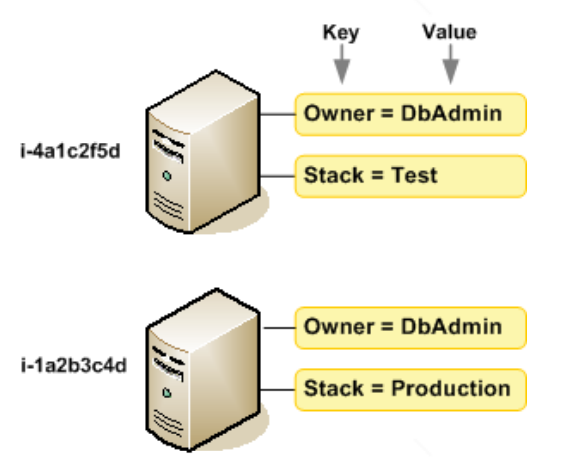
\includegraphics[scale=0.4]{sources/TagExample}
  \caption[Beispiel für ein Tag]{}\label{fig:TagExample}
Beispiel für ein Tag{\cite{AMZ26}, S.1580}.
\end{figure}
\\\\
%PAYG %https://www.nimbix.net/glossary/pay-go
\textbf{Metadaten}\\
Metadaten beschreiben andere Daten. Sie liefern Informationen über den Inhalt eines bestimmten Objekts. Ein Bild kann beispielsweise Metadaten enthalten, die beschreiben, wie groß das Bild ist, die Farbtiefe, die Bildauflösung, wann das Bild erstellt wurde und andere Daten. Die Metadaten eines Textdokuments können Informationen darüber enthalten, wie lang das Dokument ist, wer der Autor ist, wann das Dokument geschrieben wurde und eine kurze Zusammenfassung des Dokuments.
\\\\
\textbf{Startkonfiguration}\\ %https://docs.aws.amazon.com/autoscaling/ec2/userguide/create-launch-template.html
\\\\
\textbf{Scale-In/Out}\\
\\\\
\textbf{Maschinelles Lernen}\\
%Governance, Compliance ?
%\\\\
